
% ===========================
\chapter{Umsetzung}
\label{umsetzung}
% ===========================

Lorem ipsum dolor sit amet, consetetur sadipscing elitr, sed diam nonumy eirmod tempor invidunt ut labore et dolore magna aliquyam erat, sed diam voluptua.


\begin{lstlisting}[language=Python]
import numpy as np
# This is a comment
a = 5
for x in range(a):
   print("Hello")
\end{lstlisting}


Dropout - \cite{hinton2012improving}


% ===========================
\section{Definition der Fahrszenarien}
\label{umsetzung_definition}
% ===========================

In diesem Abschnitt werden Szenarien, wie in Abschnitt \ref{grundlagen_fahren_szenarien} beschrieben, als \textit{logische Szenarien} für das weitere Vorgehen in dieser Arbeit definiert. In Anlehnung an bestehende Arbeiten zu Erkennung von Fahrszenarien und auf Basis von Machbarkeitsabschätzungen für die Umsetzung werden in dieser Arbeit die Szenarien \textit{free cruising}, \textit{approaching} \textit{following}, \textit{catching up}, \textit{overtaking}, \textit{lane change left} und \textit{lane change right} auf der Autobahn betrachtet. Die Autobahn wurde ausgewählt, weil es weniger Parameter zu betrachten gibt als auf anderen Straßen wie beispielsweise in der Stadt. In der folgenden Tabelle \ref{tab_definition_szenarios} werden diese Szenarien auf \textit{funktionaler} und \textit{logischer Ebene} definiert.

Um die Darstellung in der Tabelle zu erleichtern werden folgende Abstände zwischen Ego-Fahrzeug und Fahrzeug 2 definiert. Dabei beschreibt $ego_v$ die Geschwindigkeit des Ego-Fahrzeugs in [km/h].

\begin{equation*}
\begin{split}
s_0 = ego_v * h \qquad \text{[m]} \\
s_1 = ego_v * h * \frac{2}{3} \qquad \text{[m]} \\
s_2 = ego_v * h * \frac{1}{3} \qquad \text{[m]} \\
\end{split}
\end{equation*}

\small
\begin{longtable}[c]{p{1.5cm} p{6cm} p{6cm}}
\textbf{Szenario} & \textbf{Funktionale Definition} & \textbf{Logische Definition} \\
\hline
\endhead

\textbf{Alle} & 2-spurige Autobahn geradeaus oder in einer Kurve, Geschwindigkeitsbegrenzung ist größer als 80 km/h & Breite Fahrstreifen [2,3..3,5] m \newline Geschwindigkeitsbegrenzung [80..keine] km/h \\
\hline

\textbf{Alle} & Tageslicht, keine Wolken bis leicht bewölkt, kein Niederschlag, gute Sichtbedingungen & Tageszeit [Sonnenaufgang..Sonnenuntergang] \newline Bewölkung [leicht bewölkt..wolkenlos]\\
\hline \hline

\textbf{Free cruising} & Ego, andere Verkehrsteilnehmer \newline \underline{Interaktion:} Ego fährt frei auf linker oder rechter Fahrspur, andere Fahrzeuge sind weit entfernt und haben keinen Einfluss auf die Manöver des Ego & Geschwindigkeit Ego [60..200] km/h \newline Abstand zu anderen Verkehrsteilnehmern [$>s_0$] m \\
\hline

\textbf{Approaching} & & \\
\hline

\textbf{Following} & Ego, andere Verkehrsteilnehmer \newline \underline{Interaktion:} Ego fährt auf linker oder rechter Fahrspur in sicherem Abstand hinter Fahrzeug 2 & Geschwindigkeit Ego [60..200] km/h \newline Geschwindigkeitsdifferenz zwischen Ego und Fahrzeug 2  [$<ego_v*0,05$] km/h \newline Abstand Ego zu Fahrzeug 2 [$s_2$..$s_1$] m \newline Ego befindet sich auf gleicher Fahrspur hinter Fahrzeug 2 \\
\hline

\textbf{Catching up} & Ego, andere Verkehrsteilnehmer \newline \underline{Interaktion:} Ego fährt auf linker Fahrspur und verringert den vertikalen Abstand zu Fahrzeug 2 auf der rechten Fahrspur (auf-/überholen) & Geschwindigkeit Ego [60..200] km/h \newline Geschwindigkeit Fahrzeug 2 [$<ego_v$] \newline Vertikaler Abstand Ego zu Fahrzeug 2 [0..$s_0$] m \newline Ego fährt auf linker Fahrspur hinter Fahrzeug 2 das auf rechter Fahrspur fährt \\
\hline

\textbf{Overtaking} & & \\
\hline

\textbf{Lane change left} & Ego, andere Verkehrsteilnehmer sind optional \newline \underline{Interaktion:} Ego fährt auf rechter Fahrspur und wechselt auf linke Fahrspur & Geschwindigkeit Ego [60..200] km/h \newline Ego befindet sich auf rechter Fahrspur und wechselt auf linke Fahrspur \\
\hline

\textbf{Lane change right} & Ego, andere Verkehrsteilnehmer sind optional \newline \underline{Interaktion:} Ego fährt auf linker Fahrspur und wechselt auf rechte Fahrspur & Geschwindigkeit Ego [60..200] km/h \newline Ego befindet sich auf linker Fahrspur und wechselt auf rechte Fahrspur \\
\hline

\caption{Definition der Szenarien \textit{free cruising}, \textit{following}, \textit{catching up}, \textit{lane change left} und \textit{lane change right}}
\label{tab_definition_szenarios}
\end{longtable}
\normalsize

% ===========================
\section{Generierung synthetischer Daten}
\label{umsetzung_daten_synth}
% ===========================

Auf Basis der Definitionen aus dem vorherigen Abschnitt \ref{umsetzung_definition} werden in diesem Abschnitt die benötigten Signal- und Bilddaten simuliert und entsprechend gelabelt. Dafür werden in Abschnitt \ref{umsetzung_daten_synth_simulation} die Signaldaten, die für die eindeutige Klassifizierung der Szenarien benötigt werden, simuliert. In Abschnitt \ref{umsetzung_daten_synth_labeling} werden diese Signaldaten verwendet um die parallel simulierten Bilddaten entsprechend zu labeln.
 
% ===========================
\subsection{Simulation mit CarMaker}
\label{umsetzung_daten_synth_simulation}
% ===========================

Für die Simulation der Signal- und Bilddaten wird die kommerzielle Software CarMaker von IPG Automotive \cite{ipg2018carmaker} verwendet. Diese Simulationssoftware wird für den virtuellen Fahrversuch und \ac{HiL}-Tests eingesetzt um Komponenten in unterschiedlichen Szenarien zu testen. In dieser Arbeit wird CarMaker verwendet, um die Szenarien \textit{free cruising}, \textit{following}, \textit{catching up}, \textit{lane change left} und \textit{lane change right} zu simulieren. 

Für die Aufnahme der benötigten Bilddaten wird im simulierten Fahrzeug ein entsprechender Kamerasensor konfiguriert. Die Konfiguration des Sensors orientiert sich an der Konfiguration von realen Frontview-Kameras im Fahrzeug nach Punke \cite{punke2015kamera}. So ist der Kamerasensor an der Stelle des Rückfahrspiegels platziert und hat eine Auflösung von 640x480 Pixeln, ein vertikales Blickfeld von XX° und ein horizontales Blickfeld von XX° \todo{Konfiguration einfügen}. Die Konfiguration und Position des Sensors im Modul \textit{CarMaker - Vehicle Data Set} ist in Abbildung \ref{fig_car_camera_sensor} zu sehen.

\begin{figure}[h]
\centering
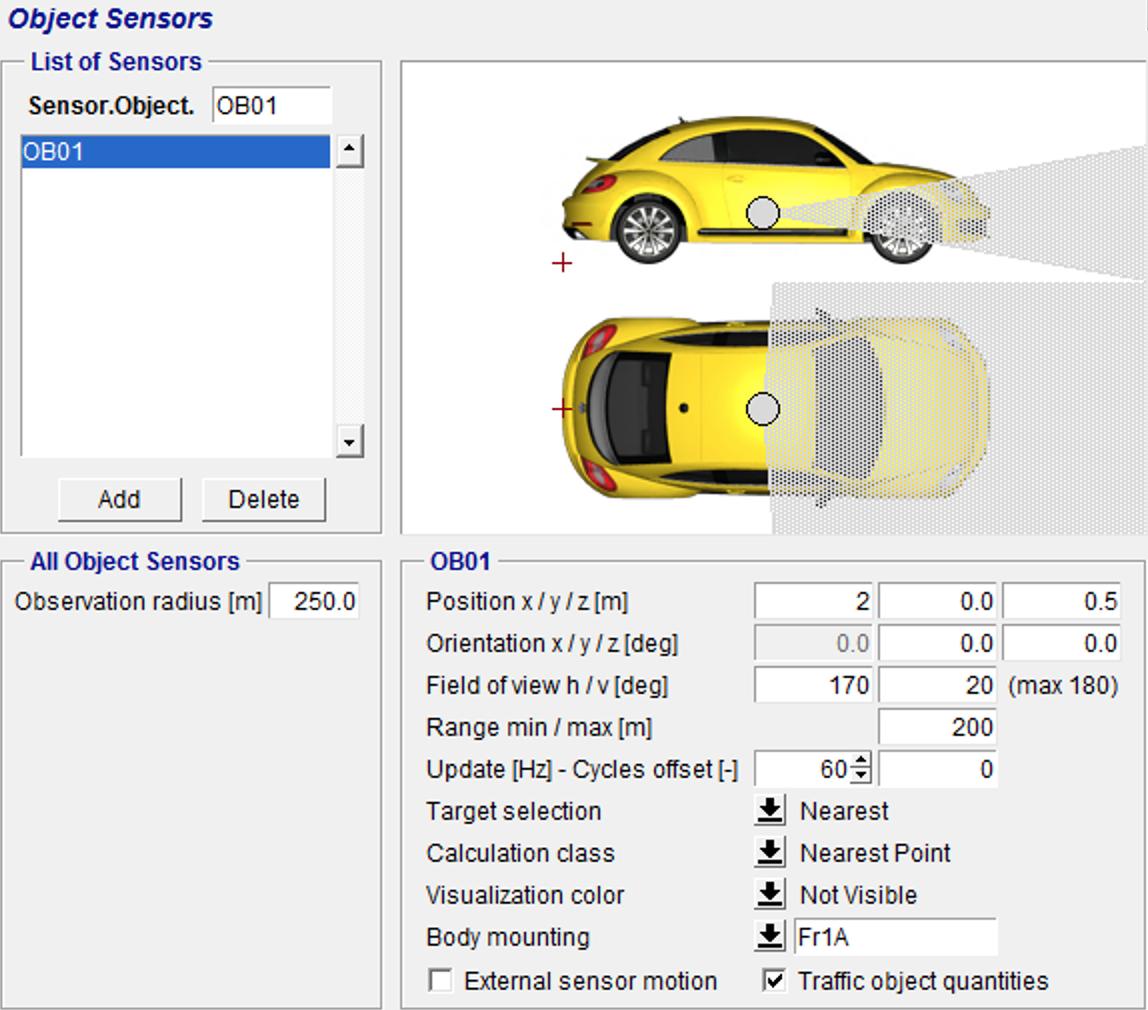
\includegraphics[scale=0.4]{car_camera_sensor.png}
\caption{Konfiguration des Kamerasensors im Modul \textit{CarMaker - Vehicle Data Set} \cite{ipg2018carmaker}}
\label{fig_car_camera_sensor}
\end{figure}

Die benötigten Signaldaten für das Labeln werden von den Definitionen aus Abschnitt \ref{umsetzung_definition} abgeleitet. Für die eindeutige Identifikation der logischen Szenarien werden die folgenden Werte benötigt: Geschwindigkeit des Ego-Fahrzeugs, Abstand und Geschwindigkeitsdifferenz des Ego-Fahrzeugs zu allen anderen Fahrzeugen, aktuelle Fahrspur des Ego-Fahrzeugs und allen anderen Fahrzeugen und die relative Position des Ego-Fahrzeugs, i.e. ob sich das Ego-Fahrzeug vor oder hinter einem anderen Fahrzeug befindet. Um den Abstand und die Geschwindigkeitsdifferenz des Ego-Fahrzeugs zu allen anderen Fahrzeugen aufzuzeichnen, wird ein Objektsensor im Ego-Fahrzeug konfiguriert. Mit diesem Sensor können im konfigurierten Radius alle Fahrzeuge und ihr Abstand und ihre relative Geschwindigkeit zum Ego-Fahrzeug erfasst und über die \textit{OutputQuantities} in CarMaker aufgezeichnet werden. Die Geschwindigkeit des Ego-Fahrzeugs und die Fahrspur-ID und Position aller Fahrzeuge können direkt, ohne zusätzlichen Sensor, über die \textit{OutputQuantities} aufgezeichnet werden. Die jeweiligen Variablen in CarMaker sind in der Tabelle \ref{tab_output_quantities} zusammengefasst.

\begin{table}[h]
\small
\centering
\def\arraystretch{1.4}
\begin{tabular}{p{6.2cm} p{7.5cm}}
\textbf{Variable in CarMaker} & \textbf{Beschreibung} \\
\hline

Car.v & Geschwindigkeit des Ego-Fahrzeugs in [m/s] \\
Car.Road.sRoad & Position des Ego-Fahrzeugs auf der Strecke in [m] \\
Car.Road.Lane.Act.LaneId & Fahrspur-ID des Ego-Fahrzeugs \\
\hline
Sensor.Object.OB01.TX.NearPnt.dv\_p & Geschwindigkeitsdifferenz zwischen Fahrzeug TX und dem Ego-Fahrzeug in [m/s] \\
Sensor.Object.OB01.TX.NearPnt.ds\_p & Abstand zwischen Fahrzeug TX und dem Ego-Fahrzeug in [m] \\
\hline
Traffic.TX.sRoad & Position des Fahrzeugs TX auf der Strecke in [m] \\
Traffic.TX.Lane.Act.LaneId & Fahrspur-ID des Fahrzeugs TX \\
\hline

\end{tabular}
\caption{Aufgezeichnete Signaldaten in CarMaker}
\label{tab_output_quantities}
\end{table}

Für die Simulation werden zwei Strecken der Länge 6.000m und 10.000m mit dem \textit{CarMaker - Scenario Editor} erstellt. Bei beiden Strecken handelt es sich um eine 4-spurige Autobahn mit zwei Fahrspuren in jede Richtung. Die Fahrtrichtungen sind in der Mitte von einer Leitplanke getrennt und am Rand der Fahrbahn sind jeweils Standstreifen vorhanden. Abschnittsweise stehen neben der Fahrbahn auch einige Bäume, was in Abbildung \ref{fig_cm_road_strecke} mit grünen Streifen gekennzeichnet ist. Abbildung \ref{fig_cm_road_bild} zeigt die Konfiguration der simulierten Straße \todo{Bild einfügen}.

\begin{figure}[h]
\centering
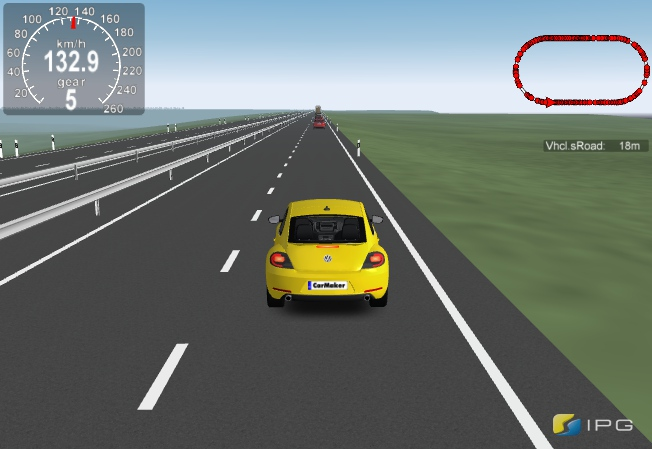
\includegraphics[scale=0.4]{cm_road_bild.jpg}
\caption{Konfiguration der simulierten Straße \cite{ipg2018carmaker}}
\label{fig_cm_road_bild}
\end{figure}

Auf beiden Strecken wird autonomer, stochastisch verteilter Verkehr erzeugt, was CarMaker mit einer gesonderten Funktion unterstützt. Der Verkehr wird in einer niedrigen Dichte (10\%) und einem 80\%-igen Anteil Autos erzeugt, andere Fahrzeuge sind Motorräder, Lastkraftwagen und Busse. In CarMaker ist eine Vielzahl an unterschiedlichen Fahrzeugen verfügbar, was wichtig ist um möglichst viele unterschiedliche Szenarien zu generieren. Mit dieser Konfiguration werden auf der 10.000m-Strecke 131 Fahrzeuge und auf der 6.000m-Strecke 89 Fahrzeuge generiert.

\begin{figure}[h]
\centering
\begin{tabular}{c}
\subfloat[Strecke 1]{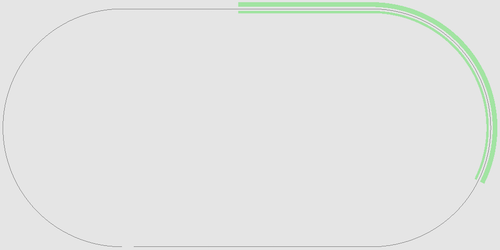
\includegraphics[scale=0.8]{cm_road_1.png}} \\
\subfloat[Strecke 2]{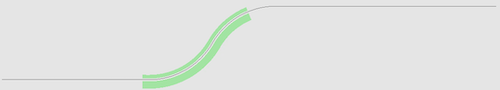
\includegraphics[scale=0.8]{cm_road_2.png}}
\end{tabular}
\caption{Schema der simulierten Strecken 1 und 2 \cite{ipg2018carmaker}}
\label{fig_cm_road_strecke}
\end{figure}

Die Simulation und Generierung von Bild- und Signaldaten wird mit dem \textit{CarMaker - Test Manager} durchgeführt. Mit diesem Modul lassen sich Fahrten mit unterschiedlichen Konfigurationen simulieren. In dieser Arbeit werden die Variablen \textit{Geschwindigkeit}, \textit{Mindestabstand zu vorausfahrendem Fahrzeug}, \textit{Minimale Geschwindigkeitsdifferenz beim Überholen} und \textit{Aggressivität beim Überholen} auf beiden oben beschriebenen Strecken variiert. Die Werte der Variablen, die simuliert werden, sind in Tabelle \ref{tab_tm_variablen} aufgelistet und sind aus der Sicht des Ego-Fahrzeugs.

\begin{table}[h]
\small
\centering
\def\arraystretch{1.4}
\begin{tabular}{p{8cm} p{0.7cm} p{0.7cm} p{0.7cm} p{0.7cm} p{0.7cm}}
\textbf{Variable} & \textbf{Werte} & & & & \\
\hline
Geschwindigkeit in [km/h] & 100 & 120 & 140 & 160 & 180 \\
Mindestabstand zu vorausfahrendem Fahrzeug in [s] & 1,0 & 1,5 & 2,0 & & \\
Minimale Geschwindigkeitsdifferenz beim Überholen in [km/h] & 5 & 15 & 25 & & \\
Aggressivität beim Überholen & 0,2 & 0,6 & 1,0 & & \\
\hline
\end{tabular}
\caption{Variablen und Werte die in der Simulation verwendet werden}
\label{tab_tm_variablen}
\end{table}

Die ersten drei Variablen sind selbsterklärend und werden hier nicht weiter erläutert. Die Variable \textit{Aggressivität beim Überholen} (in CarMaker \textit{Overtaking Rate} ist eine Zahl zwischen 0 und 1. Dabei markiert die 0 ein Fahrstil, bei dem sich der Fahrer sehr risikoavers beim Überholen verhält, i.e. Überholen nur in sehr sicheren Situationen. Je größer die Zahl wird, desto aggressiver wird der Überholvorgang und dementsprechend sinkt die Risikoaversion beim Überholen und der Fahrer überholt auch bei kritischen oder schlecht einsehbaren Situationen.

Mit diesen vier Variablen mit jeweils drei bzw. fünf Werten ergeben sich 135 verschiedene Kombinationsmöglichkeiten. Somit werden auf beiden Strecken in Summe 270 Fahrten mit 2.160 km simuliert. Signal- und Bilddaten werden mit einer Frequenz von 5 Hz aufgezeichnet, was in XXX.XXX \todo{Zahl eintragen} aufgezeichneten Szenen (Bilder und Signaldaten) resultiert. Diese Szenen werden im folgenden Abschnitt \ref{umsetzung_daten_synth_labeling} gelabelt.


% ===========================
\subsection{Daten Labeling}
\label{umsetzung_daten_synth_labeling}
% ===========================

Für das Labeln der Szenarien wird jede Szene auf Basis der Definition aus Abschnitt \ref{umsetzung_definition} mithilfe der Signaldaten klassifiziert. Die logischen Bedingungen für jedes Szenario sind dafür in Tabelle \ref{tab_logisch_labeling} aufgelistet. Auf Basis der CarMaker-Variablen aus Tabelle \ref{tab_tm_variablen} werden folgende zusätzliche Variablen definiert, um nachfolgende Bedingungen übersichtlicher darzustellen. Dabei beschreibt $v2$ jeweils das Fahrzeug, auf Basis dessen das jeweilige Szenario klassifiziert wird.

\begin{equation*}
\begin{split}
ego_v = \text{Car.v} \qquad \text{[m/s]} \\
s_0 = ego_v * h * 3,6 \qquad \text{[m]} \\
s_1 = ego_v * h * 3,6 * \frac{2}{3} \qquad \text{[m]} \\
s_2 = ego_v * h * 3,6 * \frac{1}{3} \qquad \text{[m]} \\
ego_{sRoad} = \text{Car.Road.sRoad} \qquad \text{[m]} \\
ego_{laneID} = \text{Car.Road.Lane.Act.LanId} \qquad \text{[1, 2]} \\
v2_{dv} = \text{Sensor.Object.OB01.TX.NearPnt.dv\_p} \qquad \text{[m/s]} \\
v2_{ds} = \text{Sensor.Object.OB01.TX.NearPnt.dv\_p} \qquad \text{[m]} \\
v2_{sRoad} = \text{Traffic.TX.sRoad} \qquad \text{[m]} \\
v2_{laneID} = \text{Traffic.TX.Lane.Act.LaneId} \qquad \text{[1, 2]} \\
\end{split}
\end{equation*}

\small
\begin{longtable}[c]{p{4cm} p{6cm}}
\textbf{Szenario} & \textbf{Logische Bedingungen} \\
\hline
\endhead

\textbf{Free cruising} & $ego_v > 17$ \newline $s_0 < v2_{ds}$ \\
\hline
\textbf{Following} & $v2_{dv} < ego_v * 0,05$ \newline $s_2 < s_1$ \newline $ego_{sRoad} < v2_{sRoad}$ \newline $ego_{laneID} == v2_{laneID}$ \\
\hline
\textbf{Catching up} & $v2_{dv} < 0$ \newline $0 <= v2_{ds} < s_0$ \newline $ego_{sRoad} <= v2_{sRoad}$ \newline $ego_{laneID} == v2_{laneID} - 1$ \\
\hline
\textbf{Lane change left} & $ego_{laneID}^{before} == ego_{laneID}^{after} + 1$ \newline Als Spurwechsel wird ein Intervall von 4 Sekunden betrachtet in dessen Mitte die Variable ihren Wert wechseln muss\\
\hline
\textbf{Lane change right} & $ego_{laneID}^{before} == ego_{laneID}^{after} - 1$ \newline Als Spurwechsel wird ein Intervall von 4 Sekunden betrachtet in dessen Mitte die Variable ihren Wert wechseln muss \\

\hline
\caption{Definition der Szenarien \textit{free cruising}, \textit{following}, \textit{catching up}, \textit{lane change left} und \textit{lane change right}}
\label{tab_logisch_labeling}
\end{longtable}
\normalsize

Im Anschluss an die Klassifizierung einzelner Zeitpunkte werden diese zu Szenarien zusammengefasst, wenn mindestens 15 Zeitpunkte (3 Sekunden) in Folge mit dem gleichen Label klassifiziert wurden. Insgesamt werden 326.108 Zeitpunkte und 23.972 Szenarien klassifiziert. Die Anzahl der simulierten Szenarien nach Klasse ist in der Tabelle \ref{tab_verteilung_szenarien} dargestellt. Es sind auch einige Szenarien als \textit{unknown} klassifiziert, da zwischen den definierten Szenarien andere Situationen auftreten können oder nicht die Mindestanzahl der konsekutiven Szenen erreicht wird. In einigen Zeitpunkten werden mehr als eine einzelne Szene klassifiziert. Beispielsweise kann sich das Ego-Fahrzeug gleichzeitig in der Szene \textit{catching up} und \textit{overtaking} befinden, wenn es auf der linken Fahrspur fährt und sich in vertikalem Abstand ein anderes Fahrzeug jeweils vor und hinter dem Ego-Fahrzeug befindet. 

\begin{table}[h]
\small
\centering
\def\arraystretch{1.4}
\begin{tabular}{l c}

\textbf{Szenario} & \textbf{Anzahl} \\
\hline
Free cruising & 2.545 \\
Approaching & 3.512 \\
Following & 3.601 \\
Catching up & 5.563 \\
Overtaking & 5.149 \\
Lane change left & 957 \\
Lane change right & 975 \\
Unknown & 1.670 \\
\hline
Summe & 23.972 \\
\hline

\end{tabular}
\caption{Anzahl der simulierten Szenarien nach Klasse}
\label{tab_verteilung_szenarien}
\end{table}







% ===========================
\section{Generierung realer Daten}
\label{umsetzung_daten_real}
% ===========================

Ut wisi enim ad minim veniam, quis nostrud exerci tation ullamcorper suscipit lobortis nisl ut aliquip ex ea commodo consequat.


% ===========================
\section{Training}
\label{umsetzung_training}
% ===========================

Nam liber tempor cum soluta nobis eleifend option congue nihil imperdiet doming id quod mazim placerat facer possim assum. Lorem ipsum dolor sit amet, consectetuer adipiscing elit, sed diam nonummy nibh euismod tincidunt ut laoreet dolore magna aliquam erat volutpat.


% ===========================
\subsection{Inputdaten}
\label{umsetzung_training_input}
% ===========================

Ut wisi enim ad minim veniam, quis nostrud exerci tation ullamcorper suscipit lobortis nisl ut aliquip ex ea commodo consequat. Duis autem vel eum iriure dolor in hendrerit in vulputate velit esse molestie consequat, vel illum dolore eu feugiat nulla facilisis at vero eros et accumsan et iusto odio dignissim qui blandit praesent luptatum zzril delenit augue duis dolore te feugait nulla facilisi.


% ===========================
\subsection{Architektur des neuronalen Netzes}
\label{umsetzung_training_architektur}
% ===========================

Ut wisi enim ad minim veniam, quis nostrud exerci tation ullamcorper suscipit lobortis nisl ut aliquip ex ea commodo consequat. Duis autem vel eum iriure dolor in hendrerit in vulputate velit esse molestie consequat, vel illum dolore eu feugiat nulla facilisis at vero eros et accumsan et iusto odio dignissim qui blandit praesent luptatum zzril delenit augue duis dolore te feugait nulla facilisi.


% ===========================
\subsection{Experimente}
\label{umsetzung_training_experimente}
% ===========================

 Stet clita kasd gubergren, no sea takimata sanctus est Lorem ipsum dolor sit amet. Lorem ipsum dolor sit amet, consetetur sadipscing elitr, At accusam aliquyam diam diam dolore dolores duo eirmod eos erat, et nonumy sed tempor et et invidunt justo labore Stet clita ea et gubergren, kasd magna no rebum. sanctus sea sed takimata ut vero voluptua. est Lorem ipsum dolor sit amet. Lorem ipsum dolor sit amet, consetetur

 
 

